\documentclass[border=4pt]{standalone}

\usepackage{amsmath}
\usepackage{tikz}
\usepackage{mathdots}
\usepackage{yhmath}
\usepackage{cancel}
\usepackage{color}
\usepackage{siunitx}
\usepackage{array}
\usepackage{multirow}
\usepackage{amssymb}
\usepackage{gensymb}
\usepackage{tabularx}
\usepackage{booktabs}
\usetikzlibrary{fadings}
\usetikzlibrary{patterns}


\begin{document}
 
     



\tikzset{every picture/.style={line width=0.75pt}} %set default line width to 0.75pt        

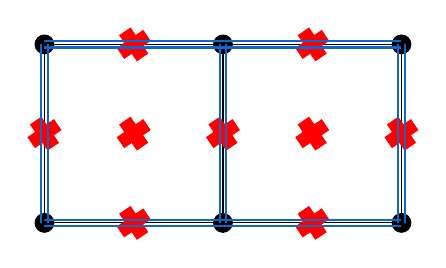
\begin{tikzpicture}[x=0.75pt,y=0.75pt,yscale=-1,xscale=1]
%uncomment if require: \path (0,543); %set diagram left start at 0, and has height of 543

%Shape: Grid [id:dp2273078730062048] 
\draw  [draw opacity=0] (142,159) -- (318.18,159) -- (318.18,250) -- (142,250) -- cycle ; \draw   (142,159) -- (142,250)(228,159) -- (228,250)(314,159) -- (314,250) ; \draw   (142,159) -- (318.18,159)(142,245) -- (318.18,245) ; \draw    ;
%Shape: Circle [id:dp8116268041258901] 
\draw  [color={rgb, 255:red, 0; green, 0; blue, 0 }  ,draw opacity=1 ][fill={rgb, 255:red, 0; green, 0; blue, 0 }  ,fill opacity=1 ] (137.5,159) .. controls (137.5,156.51) and (139.51,154.5) .. (142,154.5) .. controls (144.49,154.5) and (146.5,156.51) .. (146.5,159) .. controls (146.5,161.49) and (144.49,163.5) .. (142,163.5) .. controls (139.51,163.5) and (137.5,161.49) .. (137.5,159) -- cycle ;
%Shape: Circle [id:dp3870458790751763] 
\draw  [color={rgb, 255:red, 0; green, 0; blue, 0 }  ,draw opacity=1 ][fill={rgb, 255:red, 0; green, 0; blue, 0 }  ,fill opacity=1 ] (137.5,245) .. controls (137.5,242.51) and (139.51,240.5) .. (142,240.5) .. controls (144.49,240.5) and (146.5,242.51) .. (146.5,245) .. controls (146.5,247.49) and (144.49,249.5) .. (142,249.5) .. controls (139.51,249.5) and (137.5,247.49) .. (137.5,245) -- cycle ;
%Shape: Circle [id:dp5555208273357009] 
\draw  [color={rgb, 255:red, 0; green, 0; blue, 0 }  ,draw opacity=1 ][fill={rgb, 255:red, 0; green, 0; blue, 0 }  ,fill opacity=1 ] (223.5,245) .. controls (223.5,242.51) and (225.51,240.5) .. (228,240.5) .. controls (230.49,240.5) and (232.5,242.51) .. (232.5,245) .. controls (232.5,247.49) and (230.49,249.5) .. (228,249.5) .. controls (225.51,249.5) and (223.5,247.49) .. (223.5,245) -- cycle ;
%Shape: Circle [id:dp8192807990196815] 
\draw  [color={rgb, 255:red, 0; green, 0; blue, 0 }  ,draw opacity=1 ][fill={rgb, 255:red, 0; green, 0; blue, 0 }  ,fill opacity=1 ] (223.5,159) .. controls (223.5,156.51) and (225.51,154.5) .. (228,154.5) .. controls (230.49,154.5) and (232.5,156.51) .. (232.5,159) .. controls (232.5,161.49) and (230.49,163.5) .. (228,163.5) .. controls (225.51,163.5) and (223.5,161.49) .. (223.5,159) -- cycle ;
%Shape: Cross [id:dp6721026529931173] 
\draw  [color={rgb, 255:red, 255; green, 0; blue, 0 }  ,draw opacity=1 ][fill={rgb, 255:red, 255; green, 0; blue, 0 }  ,fill opacity=1 ] (189.53,152.38) -- (192.82,157.24) -- (189.18,159.71) -- (191.65,163.35) -- (186.58,166.79) -- (184.11,163.15) -- (180.47,165.62) -- (177.18,160.76) -- (180.82,158.29) -- (178.35,154.65) -- (183.42,151.21) -- (185.89,154.85) -- cycle ;
%Shape: Cross [id:dp03099502351179262] 
\draw  [color={rgb, 255:red, 255; green, 0; blue, 0 }  ,draw opacity=1 ][fill={rgb, 255:red, 255; green, 0; blue, 0 }  ,fill opacity=1 ] (189.53,195.38) -- (192.82,200.24) -- (189.18,202.71) -- (191.65,206.35) -- (186.58,209.79) -- (184.11,206.15) -- (180.47,208.62) -- (177.18,203.76) -- (180.82,201.29) -- (178.35,197.65) -- (183.42,194.21) -- (185.89,197.85) -- cycle ;
%Shape: Cross [id:dp7746034304485065] 
\draw  [color={rgb, 255:red, 255; green, 0; blue, 0 }  ,draw opacity=1 ][fill={rgb, 255:red, 255; green, 0; blue, 0 }  ,fill opacity=1 ] (275.53,152.38) -- (278.82,157.24) -- (275.18,159.71) -- (277.65,163.35) -- (272.58,166.79) -- (270.11,163.15) -- (266.47,165.62) -- (263.18,160.76) -- (266.82,158.29) -- (264.35,154.65) -- (269.42,151.21) -- (271.89,154.85) -- cycle ;
%Shape: Cross [id:dp09479005549054431] 
\draw  [color={rgb, 255:red, 255; green, 0; blue, 0 }  ,draw opacity=1 ][fill={rgb, 255:red, 255; green, 0; blue, 0 }  ,fill opacity=1 ] (275.53,195.38) -- (278.82,200.24) -- (275.18,202.71) -- (277.65,206.35) -- (272.58,209.79) -- (270.11,206.15) -- (266.47,208.62) -- (263.18,203.76) -- (266.82,201.29) -- (264.35,197.65) -- (269.42,194.21) -- (271.89,197.85) -- cycle ;
%Shape: Cross [id:dp9171584509330095] 
\draw  [color={rgb, 255:red, 255; green, 0; blue, 0 }  ,draw opacity=1 ][fill={rgb, 255:red, 255; green, 0; blue, 0 }  ,fill opacity=1 ] (146.53,195.38) -- (149.82,200.24) -- (146.18,202.71) -- (148.65,206.35) -- (143.58,209.79) -- (141.11,206.15) -- (137.47,208.62) -- (134.18,203.76) -- (137.82,201.29) -- (135.35,197.65) -- (140.42,194.21) -- (142.89,197.85) -- cycle ;
%Shape: Cross [id:dp1076053036917426] 
\draw  [color={rgb, 255:red, 255; green, 0; blue, 0 }  ,draw opacity=1 ][fill={rgb, 255:red, 255; green, 0; blue, 0 }  ,fill opacity=1 ] (232.53,195.38) -- (235.82,200.24) -- (232.18,202.71) -- (234.65,206.35) -- (229.58,209.79) -- (227.11,206.15) -- (223.47,208.62) -- (220.18,203.76) -- (223.82,201.29) -- (221.35,197.65) -- (226.42,194.21) -- (228.89,197.85) -- cycle ;
%Shape: Cross [id:dp5271083417007039] 
\draw  [color={rgb, 255:red, 255; green, 0; blue, 0 }  ,draw opacity=1 ][fill={rgb, 255:red, 255; green, 0; blue, 0 }  ,fill opacity=1 ] (318.53,195.38) -- (321.82,200.24) -- (318.18,202.71) -- (320.65,206.35) -- (315.58,209.79) -- (313.11,206.15) -- (309.47,208.62) -- (306.18,203.76) -- (309.82,201.29) -- (307.35,197.65) -- (312.42,194.21) -- (314.89,197.85) -- cycle ;
%Straight Lines [id:da13301909672705503] 
\draw [color={rgb, 255:red, 18; green, 102; blue, 202 }  ,draw opacity=1 ][line width=0.75]    (229.5,159) -- (229.5,245)(226.5,159) -- (226.5,245) ;


%Straight Lines [id:da31005523208702845] 
\draw [color={rgb, 255:red, 18; green, 102; blue, 202 }  ,draw opacity=1 ][line width=0.75]    (143.5,159) -- (143.5,245)(140.5,159) -- (140.5,245) ;


%Straight Lines [id:da46086323778426674] 
\draw [color={rgb, 255:red, 18; green, 102; blue, 202 }  ,draw opacity=1 ][line width=0.75]    (228,160.5) -- (142,160.5)(228,157.5) -- (142,157.5) ;


%Shape: Circle [id:dp18611044341332805] 
\draw  [color={rgb, 255:red, 0; green, 0; blue, 0 }  ,draw opacity=1 ][fill={rgb, 255:red, 0; green, 0; blue, 0 }  ,fill opacity=1 ] (309.5,159) .. controls (309.5,156.51) and (311.51,154.5) .. (314,154.5) .. controls (316.49,154.5) and (318.5,156.51) .. (318.5,159) .. controls (318.5,161.49) and (316.49,163.5) .. (314,163.5) .. controls (311.51,163.5) and (309.5,161.49) .. (309.5,159) -- cycle ;
%Shape: Circle [id:dp10670275532960938] 
\draw  [color={rgb, 255:red, 0; green, 0; blue, 0 }  ,draw opacity=1 ][fill={rgb, 255:red, 0; green, 0; blue, 0 }  ,fill opacity=1 ] (309.5,245) .. controls (309.5,242.51) and (311.51,240.5) .. (314,240.5) .. controls (316.49,240.5) and (318.5,242.51) .. (318.5,245) .. controls (318.5,247.49) and (316.49,249.5) .. (314,249.5) .. controls (311.51,249.5) and (309.5,247.49) .. (309.5,245) -- cycle ;
%Straight Lines [id:da5917511988199653] 
\draw [color={rgb, 255:red, 18; green, 102; blue, 202 }  ,draw opacity=1 ][line width=0.75]    (314,160.5) -- (228,160.5)(314,157.5) -- (228,157.5) ;


%Straight Lines [id:da35159418719210245] 
\draw [color={rgb, 255:red, 18; green, 102; blue, 202 }  ,draw opacity=1 ][line width=0.75]    (315.5,159) -- (315.5,245)(312.5,159) -- (312.5,245) ;


%Shape: Cross [id:dp5844201206054724] 
\draw  [color={rgb, 255:red, 255; green, 0; blue, 0 }  ,draw opacity=1 ][fill={rgb, 255:red, 255; green, 0; blue, 0 }  ,fill opacity=1 ] (189.53,238.39) -- (192.83,243.24) -- (189.18,245.71) -- (191.66,249.35) -- (186.58,252.79) -- (184.11,249.15) -- (180.47,251.61) -- (177.17,246.76) -- (180.82,244.29) -- (178.34,240.65) -- (183.42,237.21) -- (185.89,240.85) -- cycle ;
%Shape: Cross [id:dp016863907050807203] 
\draw  [color={rgb, 255:red, 255; green, 0; blue, 0 }  ,draw opacity=1 ][fill={rgb, 255:red, 255; green, 0; blue, 0 }  ,fill opacity=1 ] (275.53,238.38) -- (278.82,243.24) -- (275.18,245.71) -- (277.65,249.35) -- (272.58,252.79) -- (270.11,249.15) -- (266.47,251.62) -- (263.18,246.76) -- (266.82,244.29) -- (264.35,240.65) -- (269.42,237.21) -- (271.89,240.85) -- cycle ;
%Straight Lines [id:da13300790227085502] 
\draw [color={rgb, 255:red, 18; green, 102; blue, 202 }  ,draw opacity=1 ][line width=0.75]    (228,243.5) -- (314,243.5)(228,246.5) -- (314,246.5) ;


%Straight Lines [id:da8969998517334596] 
\draw [color={rgb, 255:red, 18; green, 102; blue, 202 }  ,draw opacity=1 ][line width=0.75]    (142,243.5) -- (228,243.5)(142,246.5) -- (228,246.5) ;






\end{tikzpicture}
\end{document}
